\documentclass{article}
\usepackage[utf8]{inputenc}
\usepackage{amsmath}
\usepackage{amsfonts}
\usepackage{amssymb}
\usepackage{tikz}
\usepackage{pgfplots}
\usepgfplotslibrary{fillbetween}
\usetikzlibrary{patterns}
\usepackage{color}
\usetikzlibrary{decorations.markings}
\usepackage{mhchem}
\usepackage[makeroom]{cancel}
\usepackage{hyperref}
\hypersetup{
    colorlinks=true,
    linkcolor=blue,
    filecolor=magenta,      
    urlcolor=cyan,
}
 
\urlstyle{same}


\title{How Substrate and Enzyme Concentration Affect Enzyme Kinetics}
\author{MedicinalYoyos}

\begin{document}

\maketitle
\section{zero-order and first-order with respect to substrate}
This article covers the basics of Michaelis-Menten kinetics needed to understand the orders of enzyme reactions. The general reaction scheme for enzyme to product formation is as follows:
\begin{center}
\ce{{E} + {S}
<=>[k_1][k_{-1}]
\ce{ES}
<=>[k_2][k_{-2}]
\ce{EP}
<=>[k_3][k_{-3}]
\ce{E} + {P}
}\\
\end{center}
\\

We can make some assumptions about the rates in this reaction scheme. The first assumption is that $K_3 >> K_2$. If we consolidate steps 2 and 3 of the above equation, we get a relationship that we call $k_{cat}$:
\begin{equation}
    k_{cat} = \frac{k_2k_3}{k_2 + k_3}
\end{equation}

When we factor in the assumption we made above:
\begin{gather}
    k_{cat} = \frac{k_2k_3}{\cancel{k_2} + k_3} = \frac{k_2\cancel{k_3}}{\cancel{k_3}} \nonumber \\
    \implies k_{cat} \approx k_2
\end{gather}
This means we can approximate steps 2 and 3 into one step, which is called the catalytic step. The other assumption we make in Michaelis-Menten kinetics is called the \textbf{steady state approximation.} The steady state approximation assumes that the rate of enzyme substrate complex formation = the rate of enzyme substrate complex dissociation. This means $k_1 = k_{-1}$.
We can now rewrite a much simpler equation under these assumptions:

\begin{center}
\ce{{E} + {S}
<=>[k_1][k_{-1}]
\ce{ES}
->[k_{cat}]
\ce{E} + {P}
}\\
\end{center}

The Michaelis-Menten equation is derived from these assumptions. The formula is:
\begin{equation}
    V = \frac{V_{max}[S]}{K_m + [S]} \label{1}
\end{equation}

The following is a graph of a made up enzyme that follows Michaelis-Menten kinetics. This enzyme has a $K_m$ of 0.5 and a $V_{max}$ of 3, so the equation is $V=\frac{3[S]}{0.5+[S]}$.
\\
\\
\begin{center}

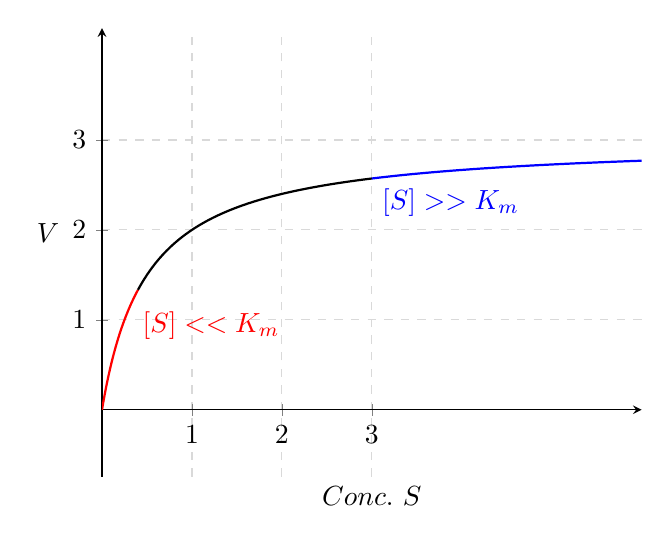
\begin{tikzpicture}

\begin{axis}[
         axis equal,
         %domain=-3:3,
         grid,
         grid style={dashed,gray!30},
         smooth,
         xmin=0, xmax=6,
         ymin=0, ymax=3.5,
         axis lines=middle,
         xlabel=$Conc.~S$,
         xlabel style={at={(axis description cs:0.5,0)},anchor=north},
         xtick={0,...,3},
         ylabel=$V$,
         ylabel style={at={(axis description cs:-0.1,.5)},anchor=south},
         ytick={0,...,3},
         samples=100,
         %legend cell align=left,
         %legend pos=outer north east,
         legend style={at={(1,1)},xshift=0cm,anchor=north east,nodes=right,fill=none}
 ]
 \addplot[red,name path=f1,mark=none,domain=0:0.4,line legend,thick] {(3*x)/(0.5+x)}
 node [pos=0.9, below right] {$[S]<<K_m$};
 
 \addplot[black,name path=f1,mark=none,domain=0.4:3,line legend,thick] {(3*x)/(0.5+x)};

 \addplot[blue,name path=f1,mark=none,domain=3:6,line legend,thick] {(3*x)/(0.5+x)}
 node [pos=0, below right] {$[S]>>K_m$};

\end{axis}

\end{tikzpicture}

\end{center}
\\

As you can see, there are two cases where the graph behaves linearly. This is when $[S]<<K_m$ and when $[S]>>K_m$. We can use these conditions to form predictive models of the rate of the reaction. In the following cases, we are going to assume that the concentration of enzyme remains constant.\\
\\
\hypertarget{case 1}{\textbf{Case 1:}} $[S]<<K_m$\\
Here, we can assume $[S] = 0$ in the denominator of the Michaelis-Menten equation \eqref{1}:\\
\begin{equation}
    V = \frac{V_{max}[S]}{K_m}
\end{equation}
Since the rate varies by the concentration only, this reaction is \textbf{first-order} with respect to $[S]$. In other words, if we consider $\frac{V_{max}}{K_m}$ to be the rate constant $k$, we find that $rate = k[S]$. We can visualize this linear relationship by thinking about how, at low concentrations of substrate, there are still enzyme binding sites that are available for more substrate. If you add 3 more substrates, 3 more binding sites are available for binding substrate even if all other substrates are bound to an enzyme. This is a linear relationship.\\
\newpage
\hypertarget{case 2}{\textbf{Case 2:}} $[S]>>K_m$\\
Here, we can assume $K_m = 0$ in the denominator of the Michaelis-Menten equation \eqref{1}:\\
\begin{align}
    V &= \frac{V_{max}\cancel{[S]}}{\cancel{[S]}} \nonumber \\
    &= V_{max}
\end{align}
Since the reaction rate does not vary with respect to substrate, this reaction is \textbf{zeroeth-order} with respect to $[S]$. Notice how the blue part of the graph is almost linear - as $[S]$ gets bigger and bigger, V gets closer and closer to $V_{max}$, which behaves like an asymptote. In other words, when $[S]$ gets really big, the rate of the reaction equals $V_{max}$. We can imagine that in this situation, all enzymes have substrate bound, and adding more substrate will not increase the rate. The only limiting factor here is the amount of enzyme and $k_{cat}$, which we will talk about in the next section.

\section{first-order and second-order with respect to substrate and enzyme}

Now let's talk about how varying the concentration of enzyme will affect the rate of the reaction. First, we need to understand the relationship between $V_{max}$ and $[E]$, which is given by the following equation:
\begin{equation}
    V_{max} = k_{cat}[E]
\end{equation}

Now we can substitute this equation into case \hyperlink{Case 1:}{1} and \hyperlink{Case 2:}{2} above and see what relationship we find:\\
\\
\textbf{Case 1:} $[S]<<K_m$
\begin{equation}
    V = \frac{k_{cat}[E][S]}{K_m}
\end{equation}
Here, the rate is \textbf{second-order} with respect to enzyme and substrate. The rate depends on both the concentration of enzyme and substrate. This is a nonlinear relationship, which I currently don't have time for so maybe I'll update this later.\\
\\
\textbf{Case 2:} $[S]>>K_m$
\begin{equation}
    V = k_{cat}[E]
\end{equation}
The rate is \textbf{first-order} with respect to enzyme and substrate. The rate \textit{only} depends on the concentration of the enzyme, and nothing else. If we revisit the example from before, all of the enzyme binding sites are filled at high concentrations of substrate. Thus, for every added enzyme, another substrate can be catalyzed. If 3 enzymes are added, 3 more substrate can be bound. This is a linear relationship.\\

In both cases, $k_{cat}$ has a direct influence on the rate of the reaction. If the $k_{cat}$ increases, the reaction rate will increase. If the $k_{cat}$ decreases, the reaction rate will increase. In fact, if we consider $[E]$ and $[S]$ to be constant and $[S] = K_m$, we get the equation for catalytic efficiency, which is the following:
\begin{equation}
    \text{Catalytic~efficiency} = \frac{k_{cat}}{K_m}
\end{equation}
In summary, because $k_{cat}$ and $K_m$ are properties of the enzyme, the enzyme is considered \textbf{more} efficient as $k_{cat}$ increases or $K_m$ decreases. The enzyme is considered \textbf{less} efficient as $k_{cat}$ decreases or $K_m$ increases.

\vspace{30mm}
Q/A:\\
\textbf{Sources/links?}\\
-my biochem notes\\
-\href{https://chem.libretexts.org/Textbook_Maps/Biological_Chemistry/Catalysts/Enzymatic_Kinetics/Michaelis-Menten_Kinetics}{LibreTexts}\\
-\href{http://www.worthington-biochem.com/introbiochem/enzymeconc.html}{Worthington Biochem}\\
-\href{https://pdfs.semanticscholar.org/presentation/dfae/6c13fda4a64a495943281d2e8efd8a2d366f.pdf}{some biochem slides from online}\\
\\
\textbf{Why did I make this?}\\
Idk for fun\\
Yes it is missing a lot of things and there are probably hella typos. I don't have time atm to be too detailed/thorough. If you'd like to view to original code, \href{https://www.overleaf.com/read/cktkpzkjxjhg}{click here}.\\
If you'd like to edit this and add stuff to it, \href{https://www.overleaf.com/4136663587tcyzzgjmrtpv}{click here}. But don't click there if you don't know latex in case something accidentally breaks, or I'll be a little sad.

\end{document}
